\documentclass[journal,12pt,twocolumn]{IEEEtran}
\usepackage{graphicx}
\graphicspath{{./figs/}}{}
\usepackage{amsmath,amssymb,amsfonts,amsthm}
\newcommand{\myvec}[1]{\ensuremath{\begin{pmatrix}#1\end{pmatrix}}}
\newcommand*{\permcomb}[4][0mu]{{{}^{#3}\mkern#1#2_{#4}}}
\newcommand*{\perm}[1][-3mu]{\permcomb[#1]{P}}
\newcommand*{\comb}[1][-1mu]{\permcomb[#1]{C}}
\usepackage{listings}
\usepackage{watermark}
\usepackage{titlesec}
\let\vec\mathbf
\providecommand{\pr}[1]{\ensuremath{\Pr\left(#1\right)}}
\providecommand{\cbrak}[1]{\ensuremath{\left\{#1\right\}}}
\providecommand{\sbrak}[1]{\ensuremath{{}\left[#1\right]}}
\providecommand{\brak}[1]{\ensuremath{\left(#1\right)}}
\providecommand{\gauss}[2]{\mathcal{N}\ensuremath{\left(#1,#2\right)}}
\providecommand{\dec}[2]{\ensuremath{\overset{#1}{\underset{#2}{\gtrless}}}}


\titlespacing{\subsection}{0pt}{\parskip}{-3pt}
\titlespacing{\subsubsection}{0pt}{\parskip}{-\parskip}
\titlespacing{\paragraph}{0pt}{\parskip}{\parskip}
\newcommand{\figuremacro}[5]{
    
}
\lstset{
frame=single, 
breaklines=true,
columns=fullflexible
}
\thiswatermark{\centering \put(0,-105.0){
\includegraphics[scale=0.4]{iith.png}} }

\sloppy
\title{\mytitle}
\title{
Digital Communication Assignment
}
\author{Nikhil Nair}
\begin{document}
\maketitle
%\tableofcontents
\bigskip


\section{\textbf{Maximum Likelihood Detection:BPSK}}
\begin{enumerate}
\item Generate equiprobable $X \in \cbrak{1,-1}$.
\item Generate 
\begin{equation}
Y = AX+N,  \nonumber
\end{equation}
where $A = 5$ dB,  and $N \sim \gauss{0}{1}$.
\item Plot $Y$ using a scatter plot.
\\

The following code  provides the solution to (1),(2) and (3) .
\\

\begin{lstlisting}
https://github.com/nikhilnair90/FWC/tree/main/Module-II/Digital_Comm/7.1/Code/7_1.py
\end{lstlisting}

\begin{figure}[h]
    \centering
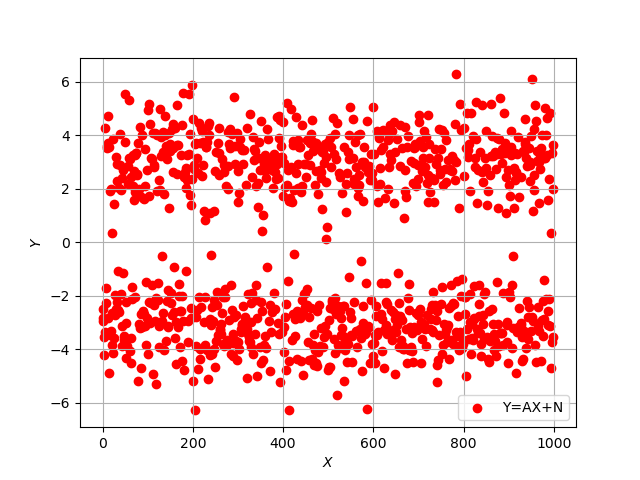
\includegraphics[width=\columnwidth]{Figure/7_1.png}
    \label{fig:Scatter plot of Y}
\end{figure}

\item Guess how to estimate $X$ from $Y$.
\\
In the question binary symbol '0' is represented as 1 and '1'  as -1
\begin{center}
0 $\longrightarrow$ 1\\
1 $\longrightarrow$ -1\\
\end{center}
Comparing the conditional pdfs of Y for X=1 and X=-1 by MAP decision rule,\\
\begin{equation}
\pr{Y | X=1} \dec{X=1}{X=-1} \pr{Y | X=-1}
\end{equation}
i.e, 
\begin{equation}
\frac{1}{\sqrt{2\pi}}\exp\brak{-\frac{(y-A)^2}{2}} \dec{1}{-1} \frac{1}{\sqrt{2\pi}}\exp\brak{-\frac{(y+A)^2}{2}}    \label{eq:2}
\end{equation}
Taking log of both sides  eq.(\ref{eq:2}) can be simplified as,
\begin{equation}
\brak{y-A}^2 \dec{1}{-1} \brak{y+A}^2 
\end{equation}
which gives the estimate of $X$ from $Y$ as,
\begin{equation}
y \dec{X=1}{X=-1} 0                  \label{eq:4}
\end{equation}
\item Find 
\begin{equation}
	P_{e|0} = \pr{\hat{X} = -1|X=1} \nonumber
\end{equation}
and 
\begin{equation}
	P_{e|1} = \pr{\hat{X} = 1|X=-1}   \nonumber
\end{equation}

From eq.(\ref{eq:4})
\begin{align}
P_{e|1}& = \pr{\hat{X} = 1|X=-1}&    \nonumber
\\
&=  \pr{Y>0|X=-1}&
\\
&=  \pr{AX+N>0|X=-1}&
\\
&=  \pr{N>A}&               \label{eq:7}
\end{align}
Q function is defined as,
\begin{equation}
Q(z) =\pr{X>z}= {\frac {1}{\sqrt {2\pi }}}\int _{z}^{\infty }e^{\frac{-x^{2}}{2}}\,dx.               \label{eq:8}
\end{equation}
where X is a  normal random variable and $\pr{X > z}$ is the probability that X is greater than z.
\\
Using eq.($\ref{eq:8}$), eq.($\ref{eq:7}$) can be re-written as
\\
\begin{equation}
P_{e|1} = Q(A)         \label{eq:9}
\end{equation}  
Similarly,
\begin{align}
P_{e|0}& = \pr{\hat{X} = -1|X=1}&    \nonumber
\\
&=  \pr{N<-A}&
\\
&= 1-Q(A)&
\\
&= Q(-A)&       \label{eq:12}
\end{align}
\\
\item Find $P_e$ assuming that $X$ has equiprobable symbols.
\\
\begin{equation}
P_e = P(0)P_{e|0}+P(1)P_{e|1}          
\end{equation} 
Since $X$ has equiprobable symbols.
\\
\begin{equation}
P_{e|0} = P_{e|1} = Q(A)        
\end{equation} 
Now,
\begin{align}
P_e &= \frac{1}{2}P_{e|0}+\frac{1}{2}P_{e|1}&
\\
&=P_{e|1}=P_{e|0}& 
\end{align}
From eq.($\ref{eq:9}$)
\begin{equation}
P_e=Q(A)
\end{equation}
\\
\item Verify by plotting  the theoretical $P_e$ with respect to $A$ from 0 to 10 dB.
\\        
\begin{figure}[h]
    \centering
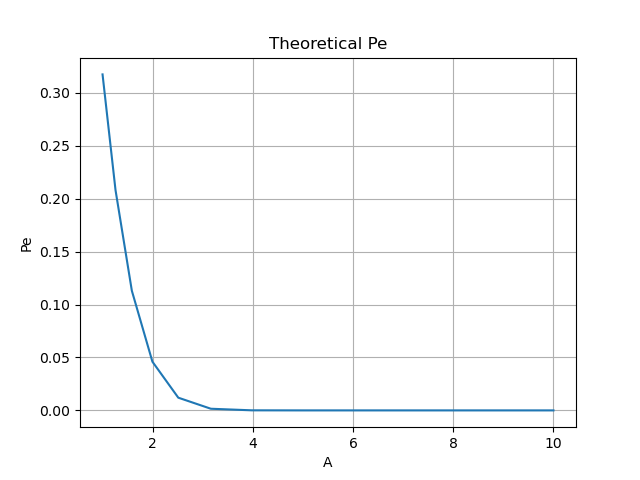
\includegraphics[width=\columnwidth]{Figure/7_1_7.png}
    \label{fig:Theoretical Pe}
\end{figure} 
\end{enumerate}



\end{document}
